\section*{2. del: bogatejši samostojni opis (21. 10. 2026)}
Nadaljevanje uporablja obstoječe izhode 1. dela (objavljen commit \texttt{7509607}); uspešni stari klici se ne ponovijo. Vsi trije delujoči modeli prejmejo iste slikovne bajte vseh 100 slik, brez referenčnih imen, ID, okvirjev ali poti anotacij. Ob izvedbi 2. dela NVILA še ni imel preverjenega slikovnega API; takrat se uporabi shranjena diagnostika brez novega prenosa ali trditve o inferenci. Kasnejši ločeni GPU zagon NVILA/Florence je dokumentiran v dodatnem nadaljevanju, kadar je prisotno.
\subsection*{Izhodna shema in dokazi}
\texttt{rich-description-v2} ohrani \texttt{scene\_description} in stare združljive podatke objektov, doda \texttt{appearance}, \texttt{image\_location}, \texttt{occlusion}, \texttt{support\_contacts}, \texttt{installation\_evidence} ter seznam \texttt{relations}. Odnos navaja začetni/ciljni lokalni ID, predikat in vidni dokaz. Validator zavrne manjkajoče podatke, podvojene ID/odnose, sklice na neobstoječe ID, samopovezave in razrede stabilnosti v prvem koraku. Neznano je izrecno \texttt{unknown}. Nobeno besedilno polje samo ne dokazuje pravilnosti trditve.
Položaji opisujejo levo/desno v sliki, ne svetovnih koordinat. Skritih vijakov, teže ali trajnosti ne zahtevamo; bližina ali negibnost ni namestitev. ID so lokalni, brez sledenja skozi čas. Napovedanih okvirjev ni; besedni položaj ni meritev natančne lokalizacije. Zato ni IoU ali mAP in na teh rezultatih še ni podlage za uvedbo posebnega detektorja.
\subsection*{Primerjava časa in oblike izhoda}
\begin{center}\small\begin{tabular}{llrrrrrrr}\toprule
Opisovalnik & Različica & OK/vsi & Med. & p90 & Povp. & Tok. & tok/s & GiB \\ \midrule
qwen35-bf16 & 1. del, podrobni & 100/100 & 4.5 & 15.4 & 7.2 & 510 & 73.3 & 8.78 \\
qwen35-bf16 & 2. del, bogati & 69/100 & 11.5 & 19.0 & 13.3 & 1130 & 87.7 & 8.78 \\
qwen35-q4 & 1. del, podrobni & 100/100 & 2.7 & 4.8 & 3.1 & 521 & 180.7 & 3.40 \\
qwen35-q4 & 2. del, bogati & 82/100 & 4.1 & 6.1 & 5.1 & 1116 & 232.7 & 3.40 \\
gemma3-q4 & 1. del, podrobni & 100/100 & 3.1 & 6.2 & 3.7 & 593 & 176.7 & 2.85 \\
gemma3-q4 & 2. del, bogati & 89/100 & 4.2 & 5.3 & 4.2 & 857 & 225.6 & 2.85 \\
\bottomrule\end{tabular}\end{center}

Časi so sekunde na sliko, tudi za zavrnjene odgovore z izmerjenim časom. Tok. je povprečje izhodnih tokenov, tok/s pa hitrost API generiranja. GiB je največja API dodelitev VRAM. Ogrevanje in nalaganje sta ločena v \texttt{part2-aggregates.json}. GPU je deljen; obremenitev in dolžina odgovora omejujeta vzročno primerjavo hitrosti. Stari prompt je podroben, novi je drugačen prompt s strožjo shemo; razlike ne pripisujemo samo strukturiranju.
Prekopirano pilotno ogrevanje ne pomeni ogretega modela po novem nalaganju. Prvi novi klic (indeks 3) posamezne skupine lahko vključuje nalaganje; celotni čas ostane v tabeli, API \texttt{load\_duration} je ohranjen ločeno. To je dodatna omejitev neposredne primerjave hitrosti, ne prikrita izločitev počasnih klicev.
\begin{center}\small\begin{tabular}{lrrrrr}\toprule
Model & Objekti & Odnosi & Opisi z odnosi & Namest. unknown & Podpora unknown \\ \midrule
qwen35-bf16 & 473 & 182 & 61/69 & 437 & 468 \\
qwen35-q4 & 539 & 218 & 82/82 & 513 & 539 \\
gemma3-q4 & 525 & 151 & 74/89 & 330 & 523 \\
\bottomrule\end{tabular}\end{center}

Objekti in odnosi so šteti le v sprejetih opisih; zavrnitve ostanejo v imenovalcih zgornje tabele. Število odnosov/objektov in prisotnost polj merita strukturo, ne pravilnosti, priklica ali vidnih dokazov. Neznano šteje le dobesedni \texttt{unknown}, ne vseh izrazov negotovosti. Vsi sprejeti odnosi imajo veljavne sklice in neprazno besedilo dokaza; ta pogoj ne potrdi vsebine fotografije.

Predhodna diagnostika prvega prompta: 1/12 po shemi, 6 ločenih ogrevanj. Zaradi izpuščenih tipov je dodana izrecna JSON tipovna predloga brez vsebinskih primerov; validator in generacijske nastavitve niso razrahljani. Diagnostični odgovori so ohranjeni ločeno in niso prišteti končni primerjavi; ne gre za prikrito popravljanje izhodov.

\newpage
\section*{2. del: vpliv opisov na besedilno presojo}
Isti izbor 10+10 slik ostane zamrznjen. Razvrščevalnik Qwen BF16 dobi celoten shranjeni opis, strukturirane objekte in odnose, brez odpiranja fotografije. Uporabljen je isti kratki prompt brez primerov iz 1. dela pri T=.3, seed 42; izbran je zaradi uspešne izpolnitve sheme, ne potrjene vsebinske prednosti. Stare BF16 odločitve se uporabijo ponovno, manjkajoče kontrole starih Q4/Gemma opisov se izvedejo le enkrat.
\begin{center}\small\begin{tabular}{llrrrrrr}\toprule
Opisovalnik & Vhod & OK/vsi & Preskoki & F & M & U & Med. [s] \\ \midrule
qwen35-bf16 & stari opis & 20/20 & 0 & 37 & 63 & 15 & 1.6 \\
qwen35-bf16 & bogati opis & 10/20 & 7 & 22 & 33 & 9 & 1.2 \\
qwen35-q4 & stari opis & 15/20 & 0 & 25 & 48 & 14 & 1.0 \\
qwen35-q4 & bogati opis & 15/20 & 4 & 24 & 63 & 22 & 1.4 \\
gemma3-q4 & stari opis & 18/20 & 0 & 26 & 63 & 9 & 1.0 \\
gemma3-q4 & bogati opis & 16/20 & 1 & 33 & 51 & 12 & 1.2 \\
\bottomrule\end{tabular}\end{center}

F/M/U so števila odločitev v sprejetih odgovorih. Preskok pomeni zavrnjen vhodni opis; ostane v imenovalcu vseh 20 položajev. Drugačno število objektov med starimi in novimi opisi pomeni, da skupnih ID ne moremo obravnavati kot iste instance.
\begin{center}\small\begin{tabular}{lrr}\toprule
Opisovalnik & Pari imen & Spremembe razreda \\ \midrule
qwen35-bf16 & 13 & 3 \\
qwen35-q4 & 16 & 5 \\
gemma3-q4 & 28 & 6 \\
\bottomrule\end{tabular}\end{center}

Pari so le enolična, natančno enaka imena po pretvorbi v male črke in normalizaciji presledkov v obeh veljavnih izhodih iste slike. Podvojena imena se izključijo; sinonimov in okvirjev ne ujemamo. To ni potrjeno ujemanje instanc; skupinska imena so posebej problematična. Sprememba ali strinjanje ni pravilnost. Konkretni pari, ID, SHA256 obeh opisov in oba modelova razloga so v \texttt{part2-decision-pairs.csv}.
\subsection*{Ožja kontrola prompta BF16 na istih 20 slikah}
\begin{center}\small\begin{tabular}{lrrr}\toprule
Različica opisa BF16 & OK/vsi & Med. [s] & Objekti \\ \midrule
1. del kratek & 20/20 & 3.4 & 81 \\
2. del bogati & 13/20 & 12.2 & 80 \\
\bottomrule\end{tabular}\end{center}

Oba prompta sta brez vsebinskih primerov in pri T=0, seed 42. Kratki stari opis se ponovno uporabi iz 1. dela. Nova shema in besedilo se še vedno spreminjata skupaj, zato to ni izolirana ablacija sheme. Za Q4/Gemma primerljivega starega kratkega opisa ni; dodatnih starih klicev za to ne izvajamo.
\subsection*{Obseg, revizija in ponovljivost}
Položajev glavne primerjave: 400; odgovorov 388; preskokov 12. Pilot: 12 odgovorov, od tega 12 prekopiranih v glavno primerjavo, brez ponovnega klica. Enkratnih novih merjenih odgovorov brez prve diagnostike: 388. Ločena nova ogrevanja: 16; 6 njihovih kopij se ne šteje ponovno. Revizija 24/24 skupin, kršitev 0; nespremenjenih starih odgovorov 846. Testi: 61 (OK).
End-to-end čas novih faz brez predhodne diagnostike: 41.7 min; pilotne kopije in 20 starih presoj niso šteti ponovno. Nalaganje in ogrevanje sta podrobno ločena v agregatih; warmup\_reused\_from\_pilot označi kopijo ogrevanja, new\_warmup\_calls pa dejanske nove klice. Za prihodnje sveže zagone je kopiranje ogrevanja odpravljeno; izvirne meritve in njihov nalagalni strošek ostanejo nespremenjeni.
\begin{verbatim}
bash scripts/thud_part2.sh --phase all
python3 -m llm_object_classifier.thud_part2_report --require-complete
python3 -m llm_object_classifier.thud_report
bash scripts/compile_thud_report.sh
\end{verbatim}
Surovi izhodi: \texttt{results/thud-part2/}; izvorni 1. del ostane v \texttt{results/thud-vmesno/}. Dopolnjeni pregled s fotografijami, referenčnimi okvirji, vsemi strukturami in odločitvami: \texttt{results/thud-part2/manual-review.html}. Konfiguracije, SHA256 kode, stanje Gita in modeli so v lokalnih manifestih/snapshotih. Ponovni zagon ohrani tudi zavrnitve in preskoke; spremenjeni vhodi se zavrnejo.

\newpage
\section*{2. del: dejanski primeri bogatejšega opisa}\subsection*{thud\_dense\_test50/frame-000007}\begin{center}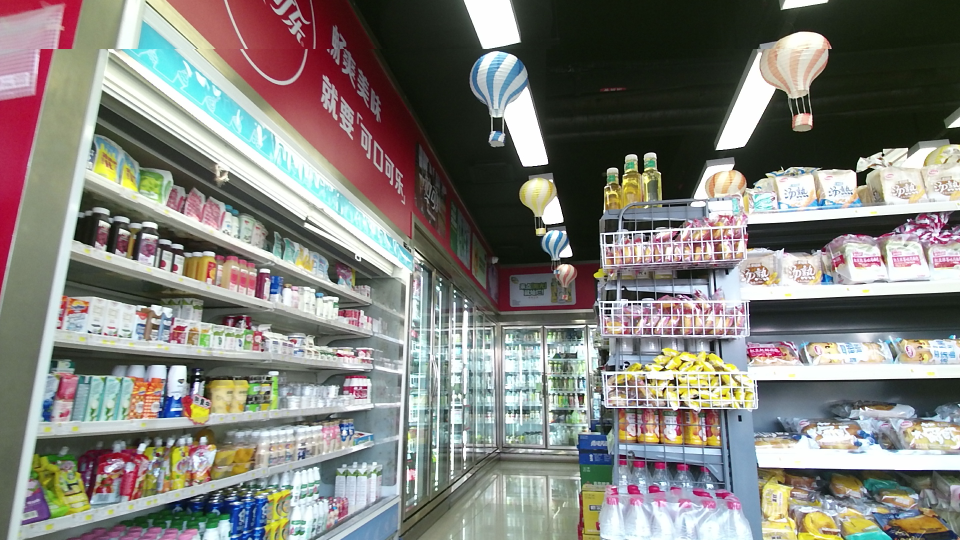
\includegraphics[height=3.2cm,width=.8\linewidth,keepaspectratio]{figures/thud_dense_test50-frame-000007.png}\end{center}\begin{center}\small\begin{tabular}{p{2.2cm}p{2.1cm}p{10.7cm}}\toprule
Model & Obj./odnosi & Dejanski prvi modelov odnos ali napaka \\ \midrule
qwen35-bf16 & zavrnjeno & Unknown relation predicate. \\
qwen35-q4 & 8/3 & refrigerated display unit beside metal shelving unit: separated by an aisle floor \\
gemma3-q4 & 5/2 & hot air balloon beside shelving unit: The hot air balloon is positioned beside the shelving unit. \\
\bottomrule\end{tabular}\end{center}
\textbf{Lastna presoja:} Q4 in Gemma pravilno postavita glavni hladilni del levo, police desno; Gemma je v starem opisu hladilnike postavila desno. Gemmina nova trditev o lesenih policah ni podprta: vidni nosilci so kovinski. Q4 navaja visible\_installation, hkrati installation\_evidence=unknown; samega vidnega znaka ne štejemo za dokaz pritrditve celotnega hladilnika. BF16 je zavrnjen zaradi above/below zunaj slovarja, ne zaradi samega prostorskega pomena. Vsi trije še združujejo izdelke. To je delni vizualni pregled.
\subsection*{thud\_dense\_test50/frame-000030}\begin{center}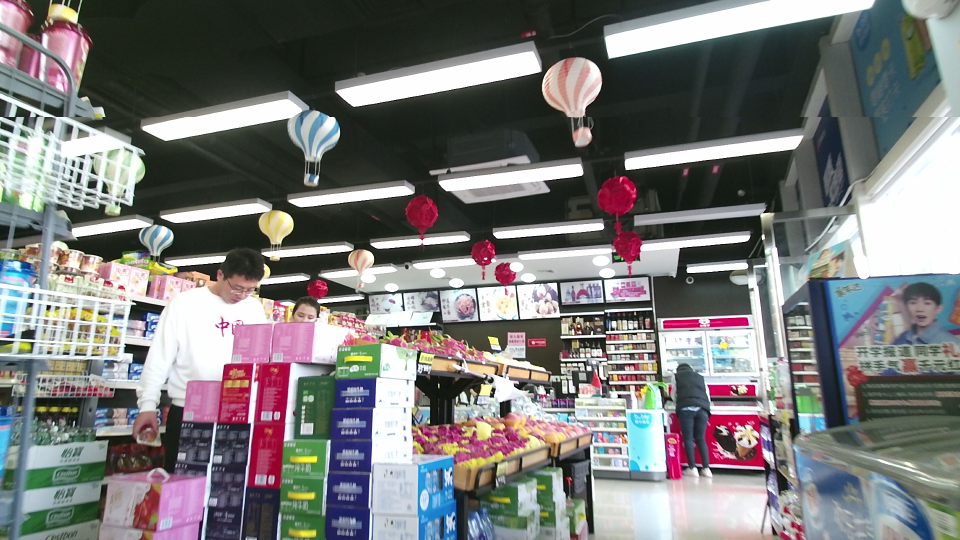
\includegraphics[height=3.2cm,width=.8\linewidth,keepaspectratio]{figures/thud_dense_test50-frame-000030.png}\end{center}\begin{center}\small\begin{tabular}{p{2.2cm}p{2.1cm}p{10.7cm}}\toprule
Model & Obj./odnosi & Dejanski prvi modelov odnos ali napaka \\ \midrule
qwen35-bf16 & 10/4 & person beside stacked boxes: standing next to stacked boxes \\
qwen35-q4 & 10/2 & person beside beverage boxes: Person stands next to stacked beverage boxes. \\
gemma3-q4 & zavrnjeno & Unknown relation predicate. \\
\bottomrule\end{tabular}\end{center}
\textbf{Lastna presoja:} BF16 zdaj loči tri osebe; delno zakrito osebo za moškim označi partial in poveže z behind, stari osnovni opis je ni izpostavil. Q4 in Gemmin zavrnjeni kandidat še navedeta le dve osebi. Referenca People ima le dve regiji, zato tega ne pretvorimo v samodejni priklic. Q4-jev razlog near the refrigerator ne podpira predikata behind. Gemmin kandidat je zavrnjen zaradi above; hkrati opis partially obscured združi z occlusion=none. Trditve BF16 o hoji iz ene fotografije ne morem potrditi. Podpore ostanejo unknown. Delni vizualni pregled, tudi zavrnjenega kandidata.
\subsection*{Dejanski besedni razlogi pri parih imen}\begin{center}\small\begin{tabular}{p{5.6cm}p{2.8cm}p{6.5cm}}\toprule
Opisovalnik / slika / ime & Staro -> bogato & Razlog modela na bogatem opisu \\ \midrule
qwen35-bf16 / agtea / image-000045 / large windows & fixed -> uncertain & Windows fixed to building but evidence is not visible. \\
qwen35-q4 / trgovina / image-000012 / refrigerated display case & uncertain -> movable & Refrigerated display case typically freestanding in retail. \\
gemma3-q4 / trgovina / image-000028 / person & movable -> uncertain & Person status varies; walking implies temporary presence. \\
\bottomrule\end{tabular}\end{center}
To so modelove utemeljitve, ne potrjena referenca; ujemanje imena ne potrdi iste instance.

\newpage
\section*{2. del: dejanski primeri bogatejšega opisa}\subsection*{thud\_agtea\_test50/frame-000002}\begin{center}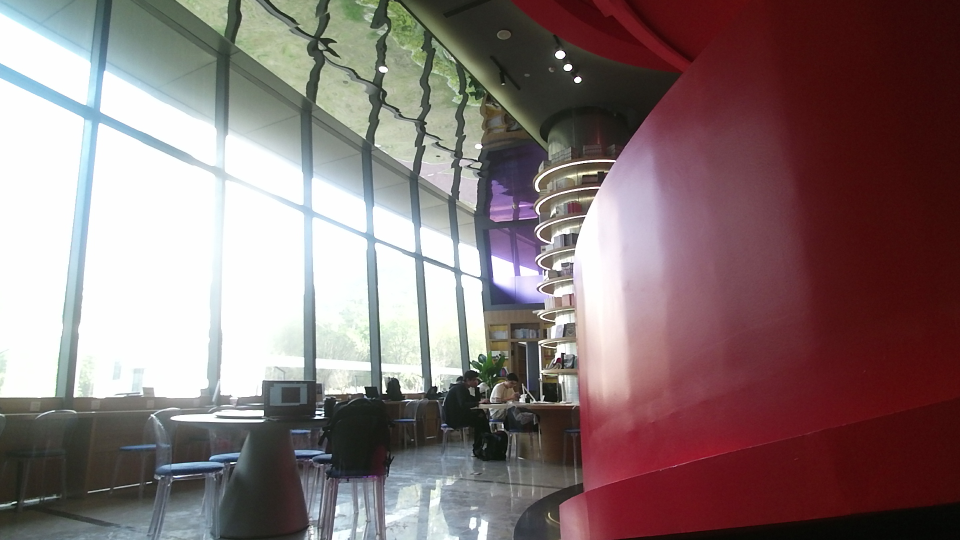
\includegraphics[height=3.2cm,width=.8\linewidth,keepaspectratio]{figures/thud_agtea_test50-frame-000002.png}\end{center}\begin{center}\small\begin{tabular}{p{2.2cm}p{2.1cm}p{10.7cm}}\toprule
Model & Obj./odnosi & Dejanski prvi modelov odnos ali napaka \\ \midrule
qwen35-bf16 & 5/0 & Brez odnosov. \\
qwen35-q4 & 5/2 & red curved structure beside spiral shelving unit: red structure is adjacent to shelving unit \\
gemma3-q4 & 6/3 & Table beside Chair: The table and chair are positioned adjacent to each other. \\
\bottomrule\end{tabular}\end{center}
\textbf{Lastna presoja:} BF16 tudi v novem veljavnem izhodu stole opiše kot transparent plastic; vidim kovinske cevne okvirje in modra sedišča. Q4 še združuje tables and chairs. Gemma okno postavi right/top/full, čeprav prevladuje na levi; vijolične svetilke, ki jo navede, ne morem potrditi. BF16 ne vrne nobenega odnosa; Q4 in Gemma vrneta odnose, vendar to še ne potrdi njihove vsebine. Pri vidnih stolih in mizah ostanejo podpore unknown. To je delni vizualni pregled, ne popolna referenca stabilnosti.
\subsection*{thud\_agtea\_test50/frame-000026}\begin{center}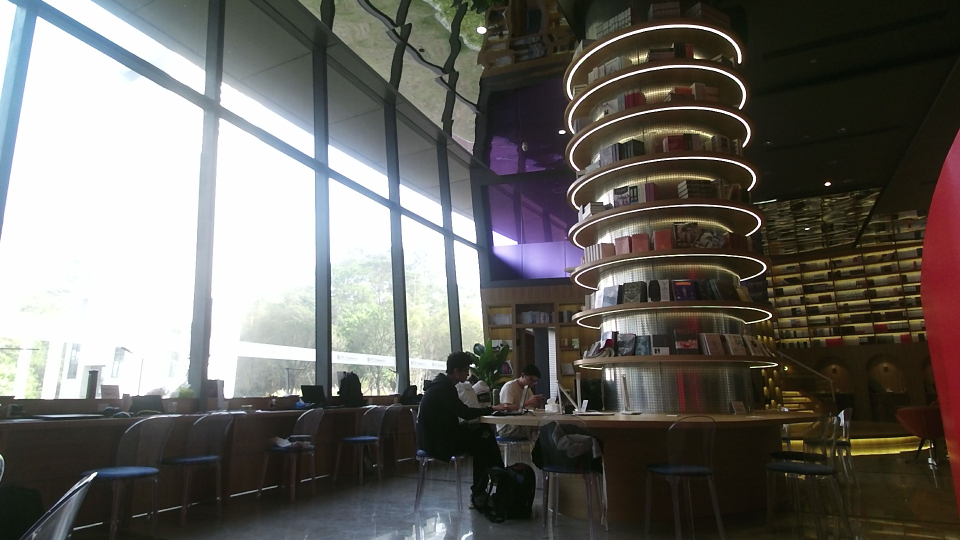
\includegraphics[height=3.2cm,width=.8\linewidth,keepaspectratio]{figures/thud_agtea_test50-frame-000026.png}\end{center}\begin{center}\small\begin{tabular}{p{2.2cm}p{2.1cm}p{10.7cm}}\toprule
Model & Obj./odnosi & Dejanski prvi modelov odnos ali napaka \\ \midrule
qwen35-bf16 & zavrnjeno & Unknown relation predicate. \\
qwen35-q4 & 8/3 & person beside person: seated next to each other at the table \\
gemma3-q4 & 6/3 & Circular Bookshelf beside Chair: The circular bookshelf is beside the chair. \\
\bottomrule\end{tabular}\end{center}
\textbf{Lastna presoja:} BF16 kandidat je zavrnjen zaradi at in near; zato ne gre v razvrščanje. Dve osebi, krožna polica in modri kovinski stoli v njem so vizualno smiselni, a zakritost vseh označi none. Q4 sprejeti opis loči dve osebi in stola z modrim sediščem; odnos miza under spiral bookshelf zahteva presojo stika in globine, ne le vertikalnega položaja. Gemma si izmisli sive pisarniške stole z nasloni za roke in drugo osebo postavi desno, čeprav sta vidni osebi levo od krožne police. Vsi ohranijo podpore unknown. Namestitve police ne morem potrditi. Delni vizualni pregled, tudi zavrnjenega kandidata.
\subsection*{Sklep in naslednji poskus}Bogatejši zapis omogoča pregled zakritosti in odnosov ter konkreten popravek pri tretji osebi v gostem prizoru. Ne potrjuje pa splošne izboljšave: sprejeti JSON še vsebuje napačne materiale, lokacije in nepodprte dokaze namestitve, številne podpore ostanejo neznane. Večja shema poveča izhod in prinese dodatne zavrnitve. Naslednji kontrolirani poskus naj na istih 20 slikah najprej razjasni slovar odnosov ob nespremenjenih drugih pogojih, nato ločeno preveri tipovno predlogo brez privzetih vrednosti unknown. Neznano mora ostati dovoljeno, kadar dokaz ni viden. Pred končno izbiro modela/prompta je potreben sistematičen ročni pregled istih objektov in stikov. Največ veljavnih JSON ni dokaz najboljše vsebine; brez referenc stabilnosti accuracy ostaja nedoločena.
